\section*{Results}
In Figure 4, we showcase our first successful keep-alive connection. Here, two threads each handle a series of requests over a single connection, rather than multiple separate connections. In Figure 5, we present our first running CGI script, which outputs dynamic data, such as the user's IP address, that cannot be generated by a static file.

\begin{figure}[h]
    \centering
    \begin{minipage}{0.5\textwidth}
        \centering
        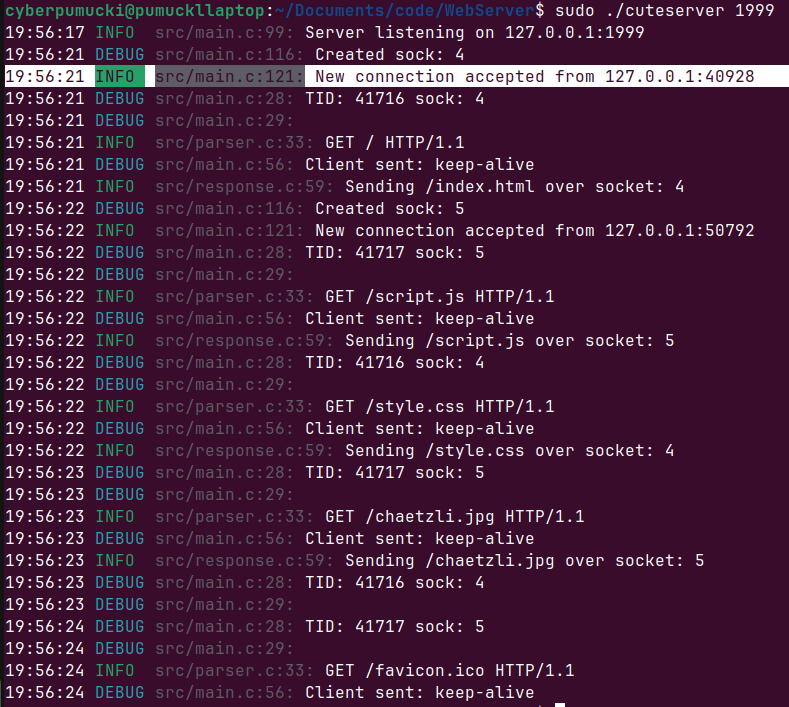
\includegraphics[width=\textwidth]{figures/keep-alive.png}
        \caption{Keep-Alive: Multiple Requests handled over one Connection}
    \end{minipage}
    \hfill
    \begin{minipage}{0.35\textwidth}
        \centering
        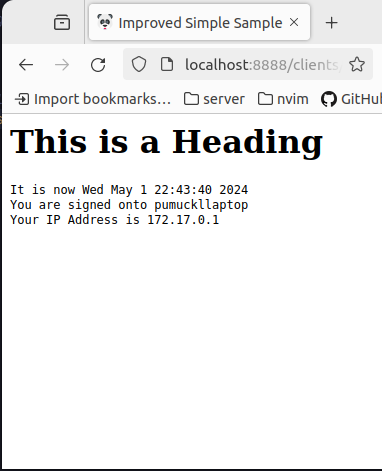
\includegraphics[width=\textwidth]{figures/cgi.png}
        \caption{First simple CGI Script with Environment Variables}
    \end{minipage}
\end{figure}
\vspace{-15pt}
\subsection*{Performance Testing}
We wanted to test the influence of the number of worker threads on the performance of our application. For this we used \textbf{Locust} \footnote{\url{https://locust.io/}} to tests POST and GET requests to our application, as well as static file requests. 

\subsubsection*{Static File Tests}
We conducted these tests using the following Locust Configuration: 500 virtual users, ramping up at 50 users/second, for a runtime of 60 seconds. Requests were made to a static file hosted on a home server with 4 cores, and multithreading was managed by OpenMP.
The graphs for 2 versus 3 worker threads (Figures 7 and 8) exhibit similar trends, so the application runs relatively stable. The graph shows an initial peak in response time, followed by a gradual decline and stabilization at lower values. We can only explain this result by assuming that the responses are being cached somewhere.
The number of requests is similar, but the average response time with 2 threads is 239.07ms, while with 3 threads, it is 154.19ms—a reduction of about 85ms. This indicates that multithreading reduces the response time per request.
\begin{figure}[h]
    \centering
    \begin{minipage}{0.45\textwidth}
        \centering
        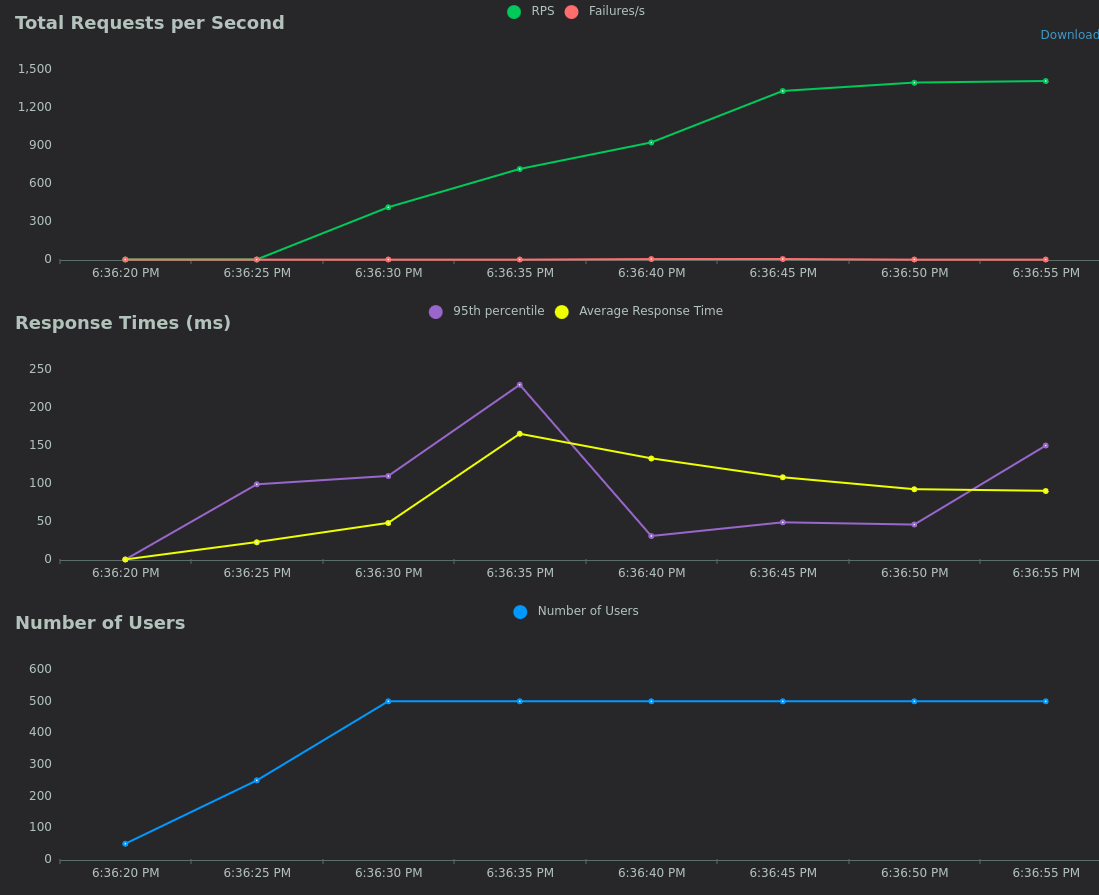
\includegraphics[width=\textwidth]{figures/2threads.png}
        % 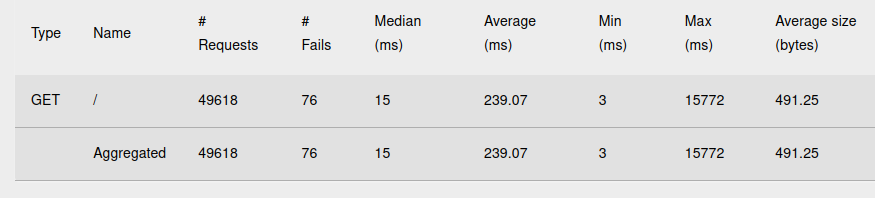
\includegraphics[width=\textwidth]{figures/2_threads_chart.png}
        \caption{Requests to a static file, 2 Threads}
    \end{minipage}
    \hfill
    \begin{minipage}{0.45\textwidth}
        \centering
        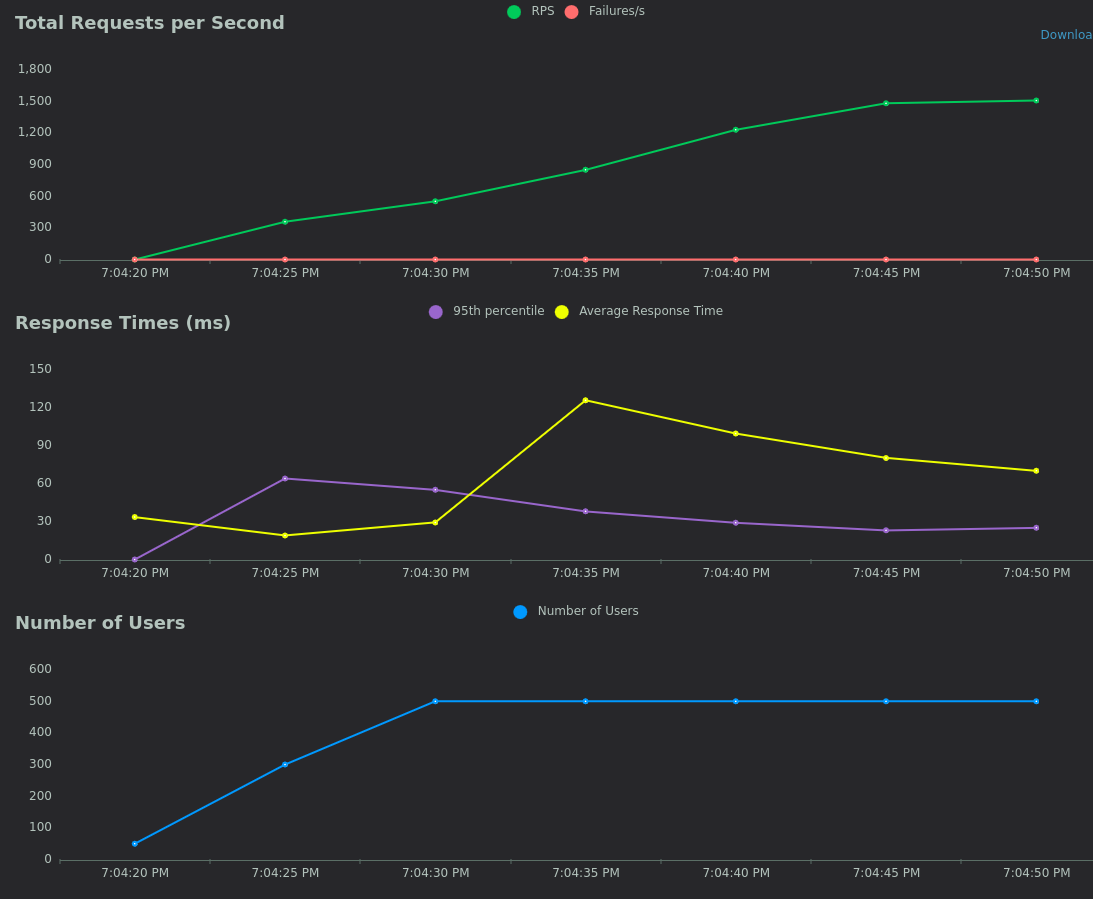
\includegraphics[width=\textwidth]{figures/3threads.png}
        % 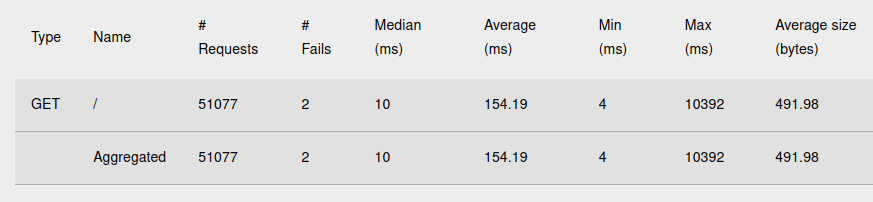
\includegraphics[width=\textwidth]{figures/3_threads_chart.png}
        \caption{Requests to a static file, 3 Threads}
    \end{minipage}
\end{figure}

\subsubsection*{CGI Tests}
We also tested the response times of requests made to CGI scripts using the same Locust configuration and hosting conditions. Under heavy load with two worker threads, the average response time was 1506.15 ms. With four threads, the average response time improved to 882.46 ms, showing a speedup of 1.7. Additionally, the number of failures decreased from 222 to 11 with four threads (See Figures 9 and 10). \footnote{Detailed results can be found in \textbackslash testing\textbackslash results relative to the project root directory}
This demonstrates a significant overall improvement when using more threads. Comparing requests to the static file with two threads, requests to the CGI script were 1267.08 ms slower. This is due to the spawning of new processes for each request in the CGI case and the additional code required for handling CGI scripts. These results would likely improve if we had implemented FastCGI.

\begin{figure}[h]
    \centering
    \begin{minipage}{0.45\textwidth}
        \centering
        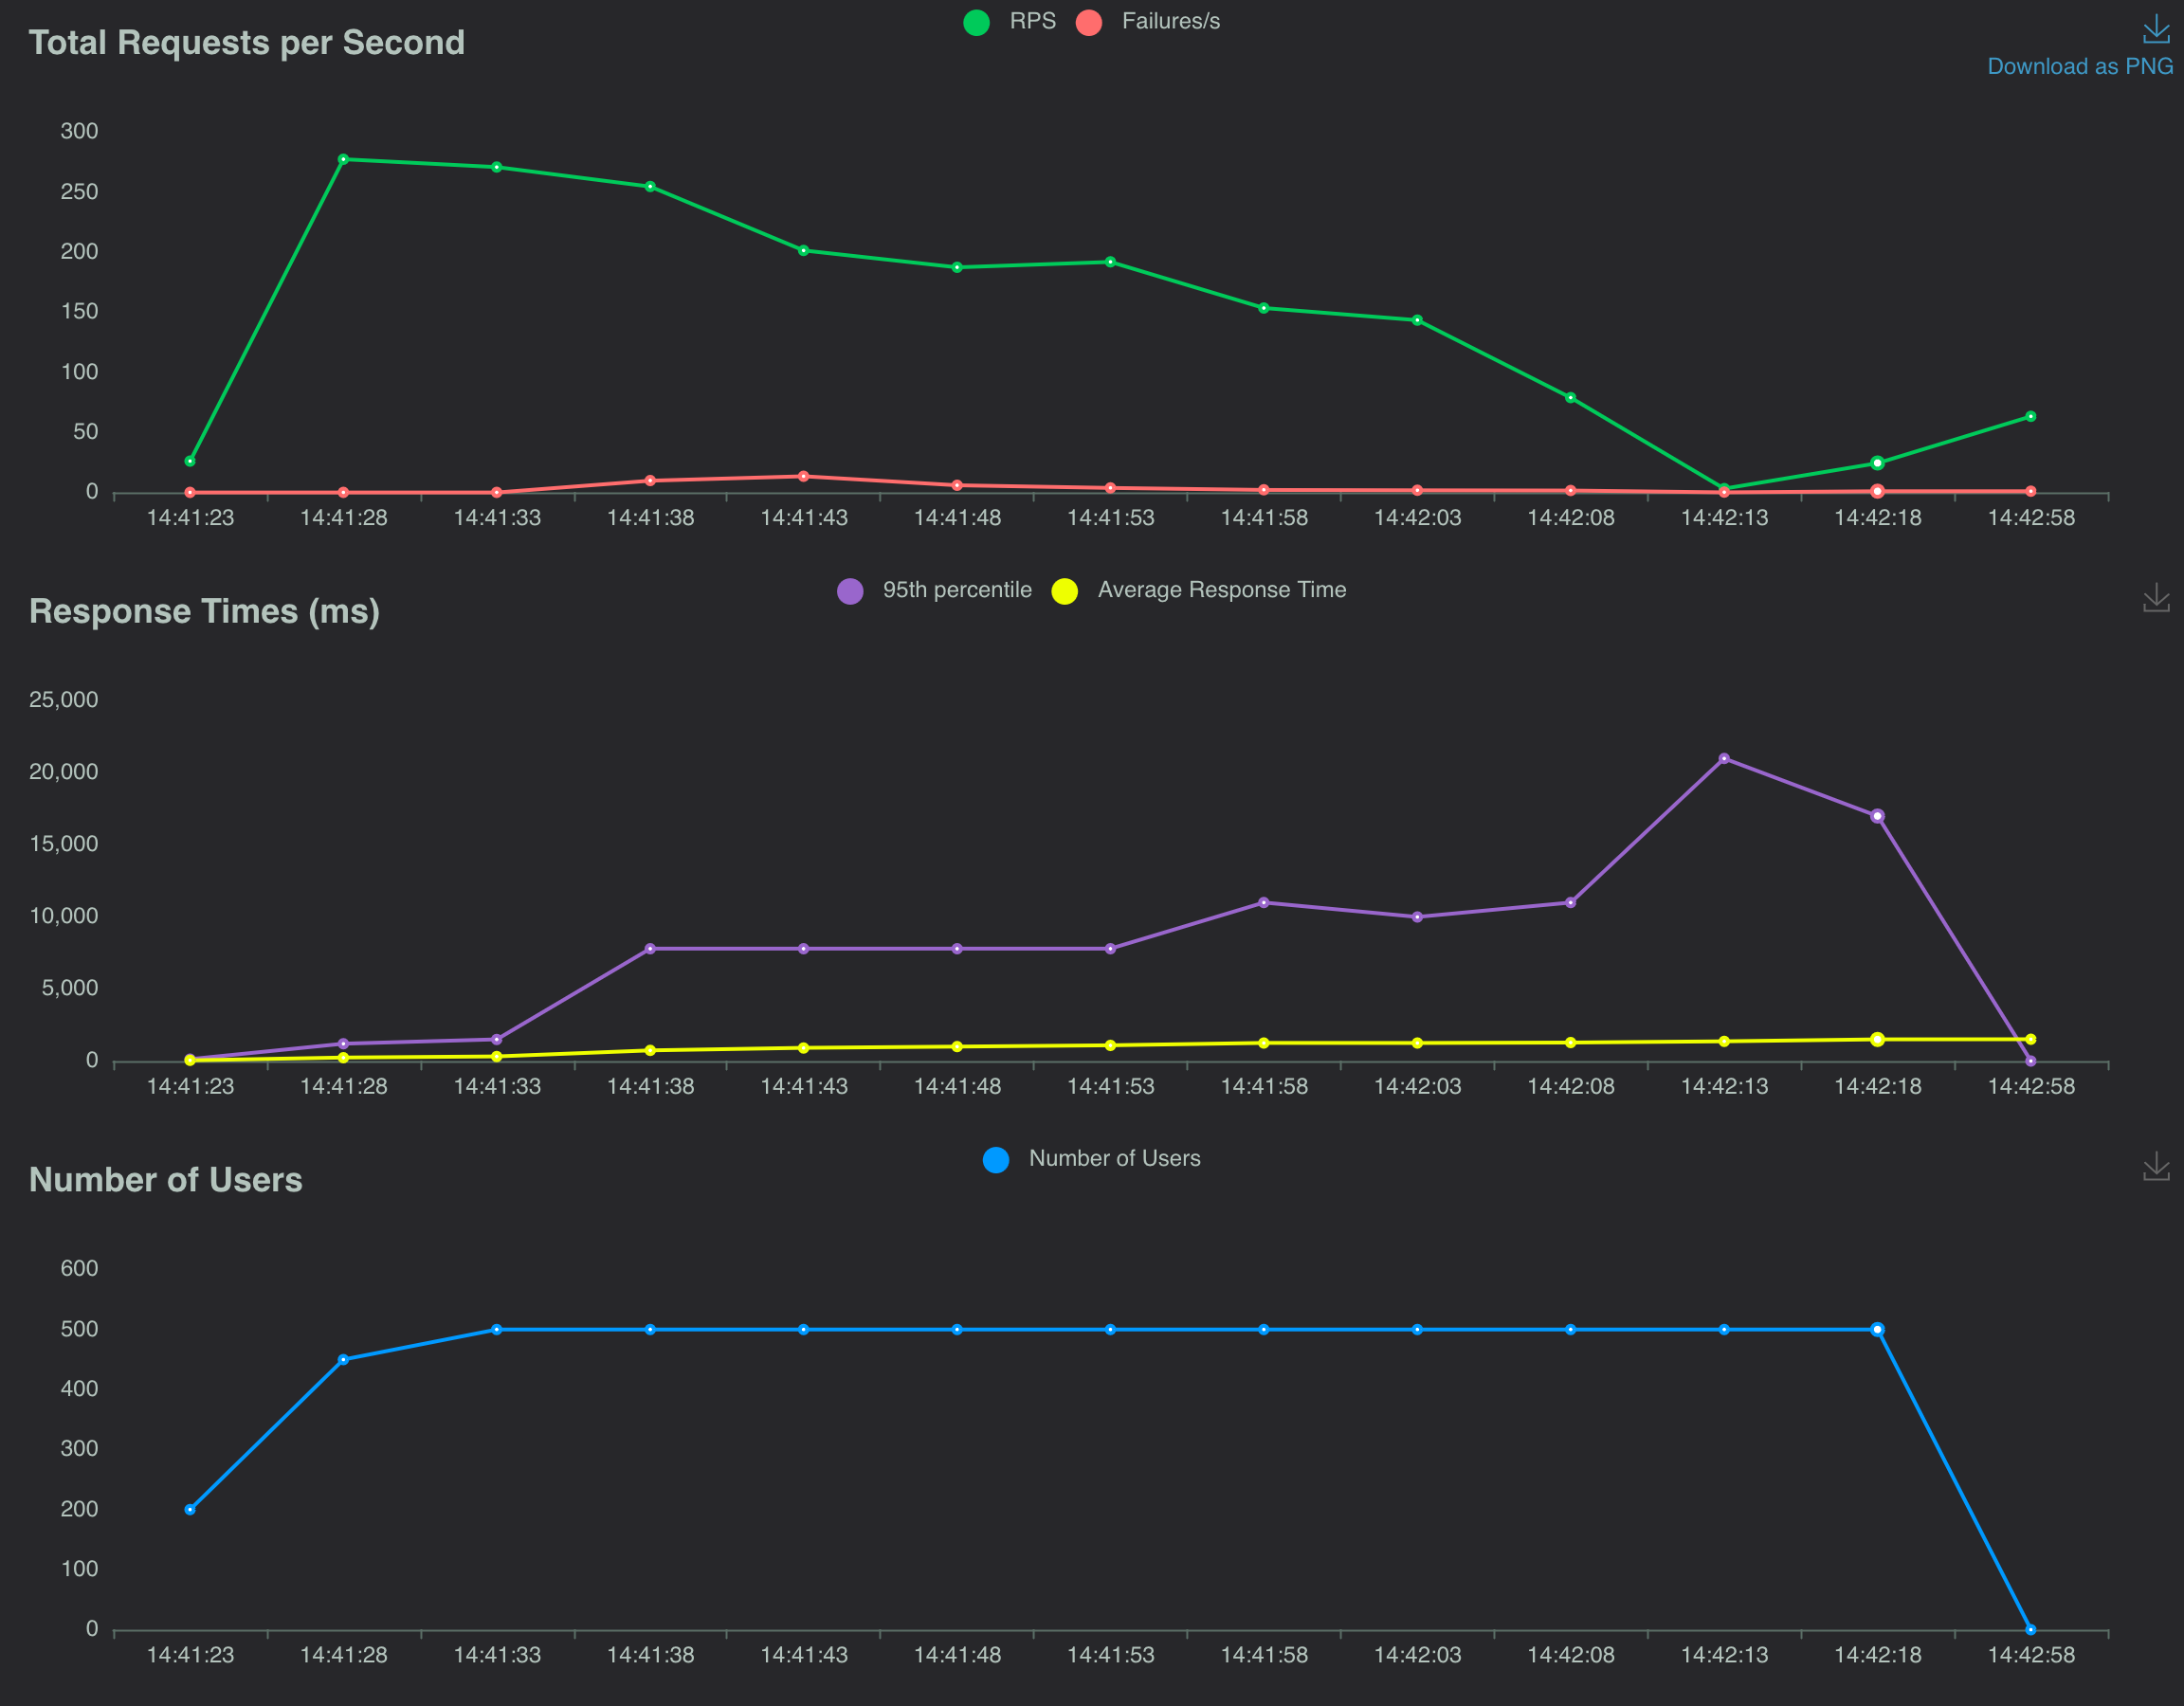
\includegraphics[width=\textwidth]{figures/cgi_2threads.png}
        \caption{Requests to a CGI script, 2 Threads}
    \end{minipage}
    \hfill
    \begin{minipage}{0.45\textwidth}
        \centering
        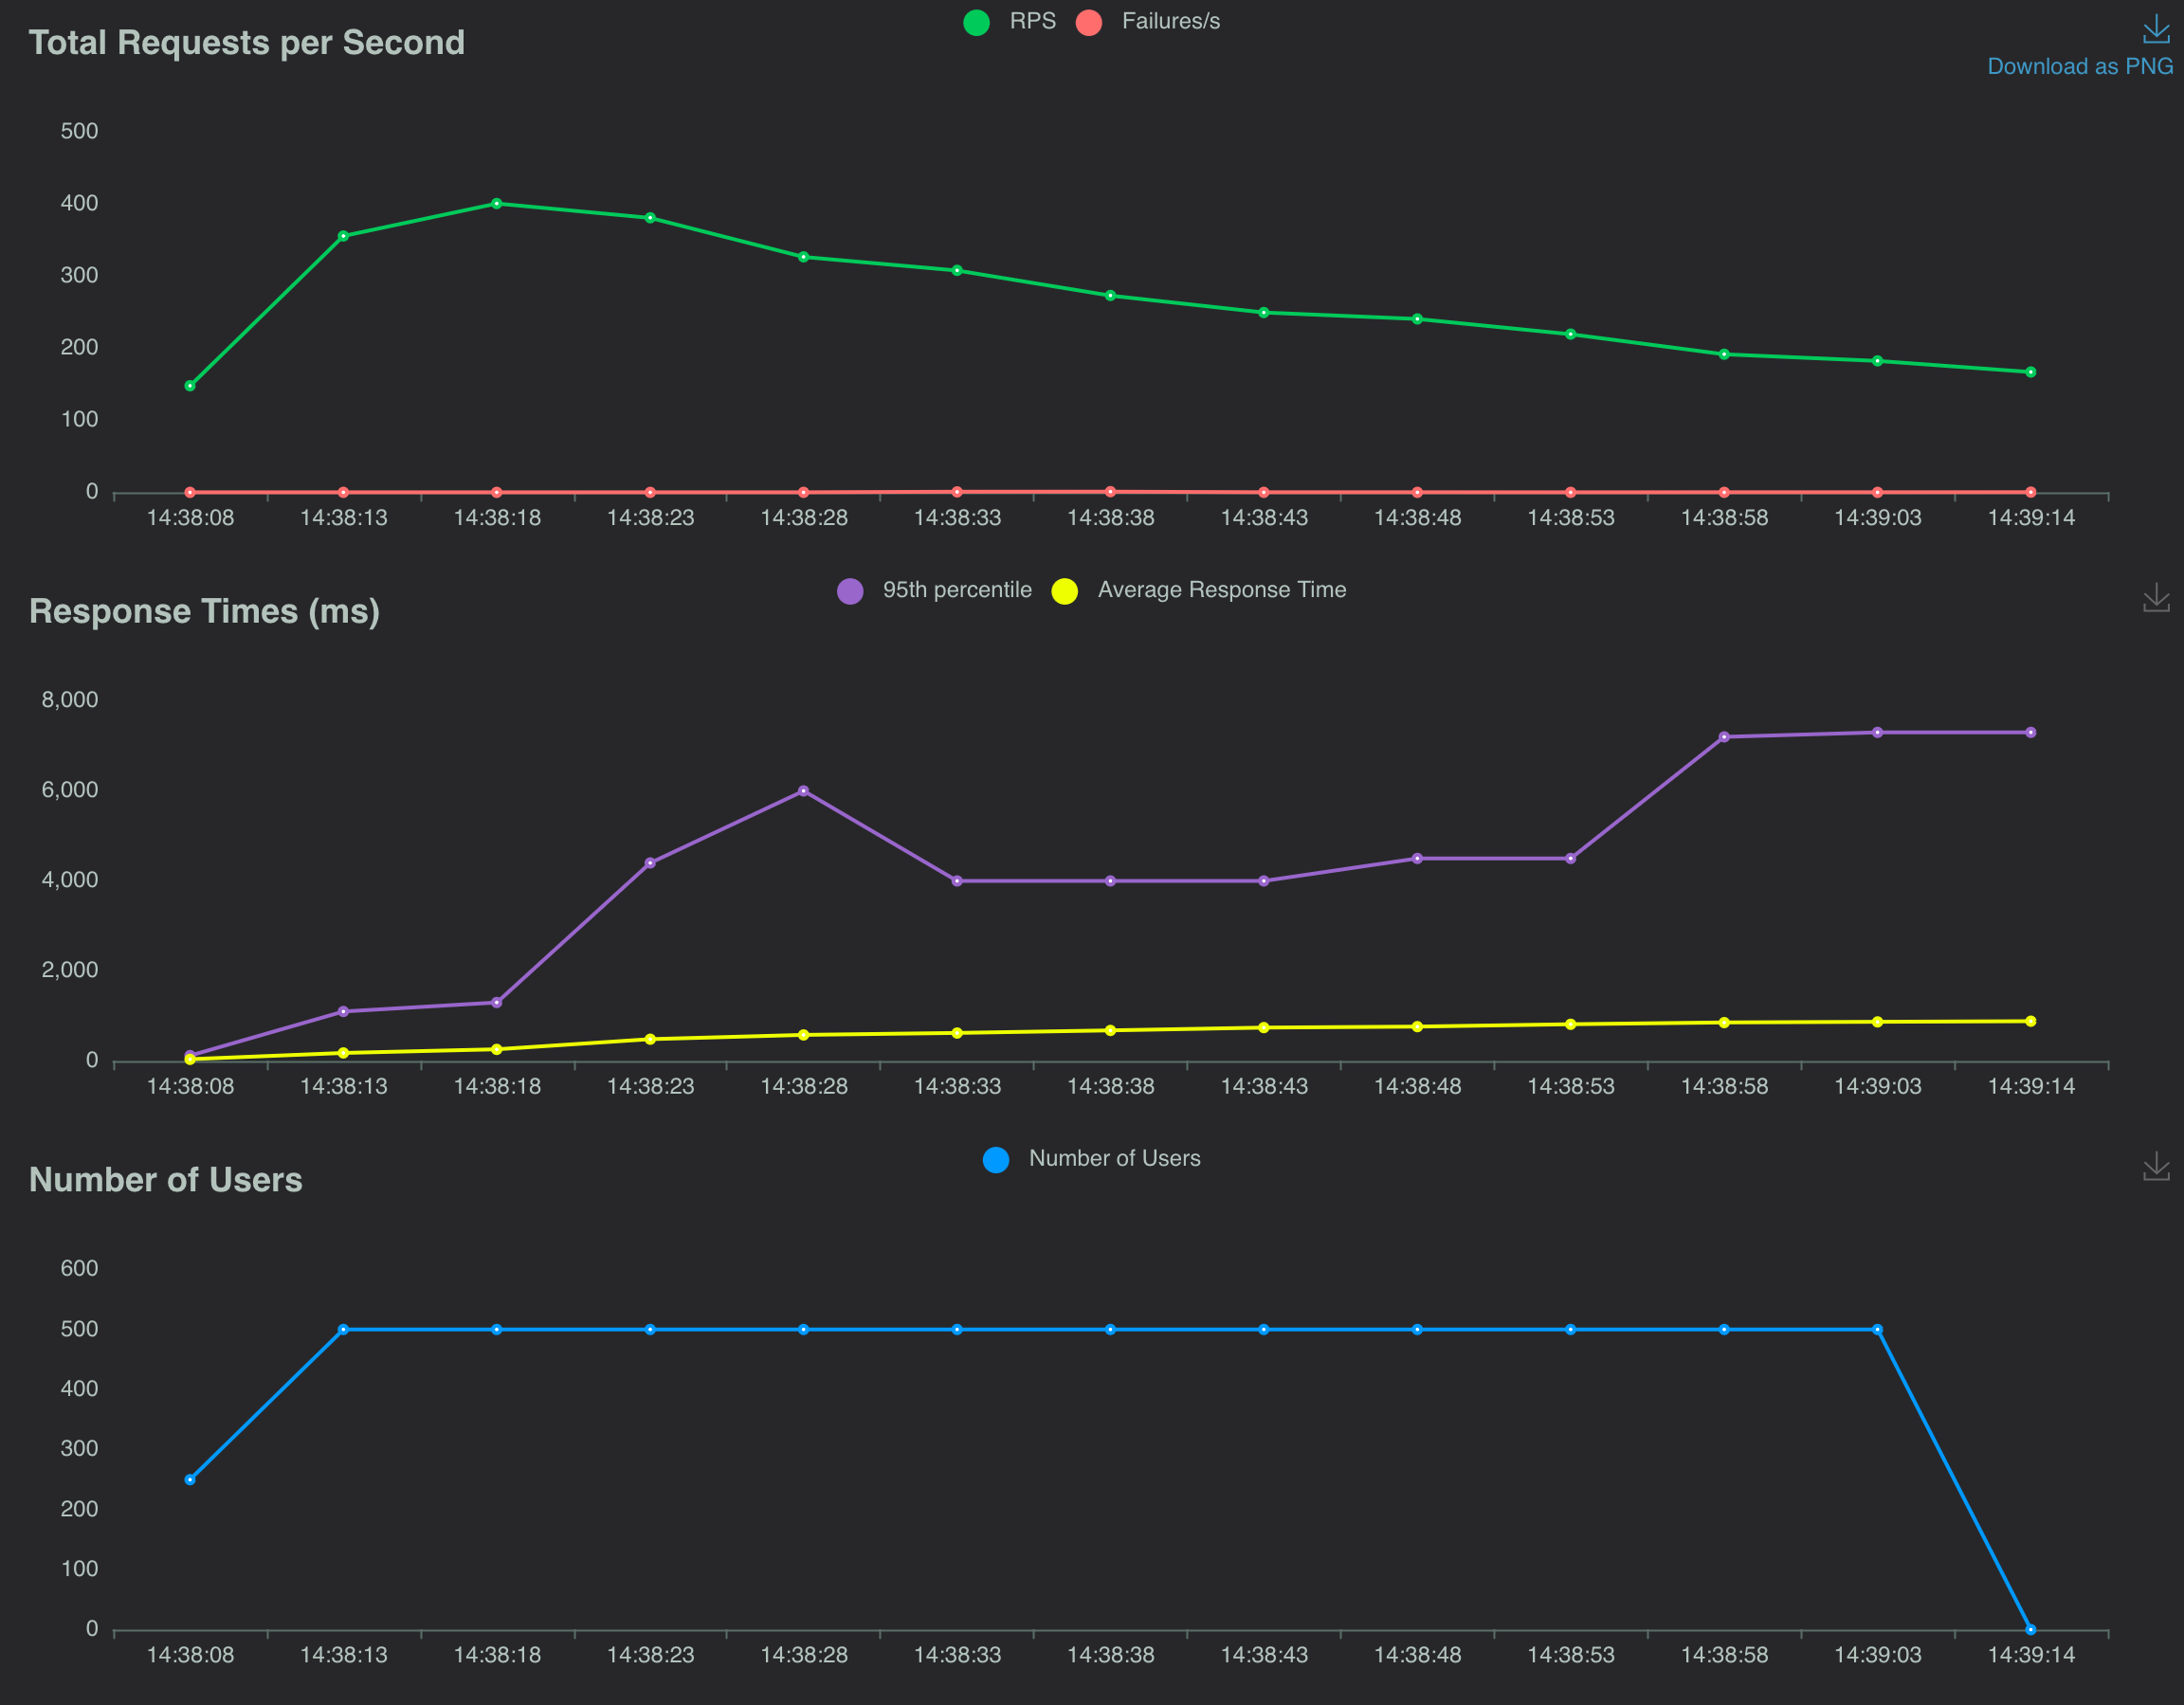
\includegraphics[width=\textwidth]{figures/cgi_4threads.png}
        \caption{Requests to a CGI script, 4 Threads}
    \end{minipage}
\end{figure}
